\documentclass[a4paper,11pt,twoside,british]{report}
% This is an annotated latex definition file.
% You can give it any name as long as its inputted somewhere
% in your code.
% You may even put it in a directory other then the current
% as long as that directory is in the TEXINPUTS path.
% Comments start with a % as you a seeing right now. Otherwise look
% to the left.
% font of the times family
\usepackage{nextpage}
\usepackage{times}
% make linenumbering possible for reviewing
\usepackage[pagewise,mathlines,displaymath]{lineno}
\usepackage[utf8]{inputenc}
% use the pdftex graphics extensions
\usepackage[pdftex]{graphicx}
%\DeclareGraphicsRule{*}{mps}{*}{}
\usepackage{picins}
\usepackage{ragged2e}
% geometry for the documents in this dir.
\usepackage[a4paper,includemp,
      scale={0.93,0.87},
      includeheadfoot,
      bindingoffset=1.2cm]{geometry}

%%% Local Variables: 
%%% mode: latex
%%% TeX-master: "sofa.tex"
%%% End: 


% to make the headers and footers look nice
\usepackage{color,fancyhdr}
% for version control info, e.g. in the header or footer
\usepackage{svn}
% make the header (and footer) span the whole printable area
\addtolength\headwidth\marginparwidth
\addtolength\headwidth\marginparsep
\pagestyle{fancy}
% to get version information in files, include the following lines in each document 
\newcommand\PartAuthor{Pieter van den Hombergh}
\newcommand\PartReviewer{Pieter van den Hombergh}
\SVN $Author: hom $
\SVN $Revision: 28 $
\SVN $Id: styledefs.tex 28 2014-09-24 09:04:24Z hom $
\SVN $Date: 2014-09-24 11:04:24 +0200 (Wed, 24 Sep 2014) $
\newcommand\TheFile{styledefs.tex}
%\renewcommand\footrulewidth{1pt}
% put revision control info in the footer
% this info comes from RCS but more likely from CVS
% the vspace compensates for the space taken up by the logo on the right hand.
% I like a fontys color in my header
\definecolor{fontys}{rgb}{0.2,0,0.2} % a darkish purple
\definecolor{purple}{rgb}{0.6,0,0.4} % a redish purple
\definecolor{navy}{rgb}{0.0,0,0.4} % a darkish blue
\renewcommand\headrule{%
  {\color{navy}%
    \hrule height 2pt width \headwidth
    \vspace{1pt}%
    \hrule height 1pt width \headwidth
    \vspace{-4pt}%
  }%
}%
\renewcommand\footrule{
  {\color{fontys}%
    \hrule height 1pt width \headwidth
    \vspace{1pt}%
    \hrule height 2pt width \headwidth
    \vspace{2pt}%
  }%
}
% do not indent pars, increase parskip
\setlength\parindent{0pt}
\setlength\parskip{0.5em}
% my own itemize: a bit less spacy then the default
\newenvironment{Itemize} {
  \begin{itemize}{}%
    \setlength\topsep{0ex}%
    \setlength\parskip{0ex}%
    \setlength\partopsep{0em}%
    \setlength\parsep{0em}%
    \setlength\itemsep{0em}%
    }%
  {\end{itemize}}
% make the head a bit heigher
\setlength\headheight{16pt}
\setlength\footskip{60pt}
% This macro '\define' puts the argument in em 
% and in boldface in the margin.
\newcommand{\Define}[1]{% 1 argument
  \mbox{}{\textit{#1}}% italics or em
  \marginpar{\raggedright% no adjust
    \bfseries\hspace{0pt}#1}% bold
} % end of macro
\newcommand\Okis[1]{{\color{fontys}\textbf{#1}}}
\newcommand\Code[1]{{\color{fontys}\texttt{#1}}}
\newcommand\Linux{{\color{fontys}\sc\bf Linux\ }}
% At start of pages, define sometimes puts the material in the wrong margin
% in that case use this fix.
\newcommand{\fixdefine}[1]{\mbox{}{\textit{#1}}%
  \reversemarginpar\marginpar{\bfseries\hspace{0pt}#1}\normalmarginpar}
% to display source code like things
\usepackage{listings}
\lstset{numbers=left} % to get out of the way with document line numbers
% to be able to 'on this page' and the like
\usepackage{varioref}
% to put a nice quote with the chapter
\usepackage[avantgarde]{quotchap}
\renewcommand\chapterheadstartvskip{\vspace*{-5\baselineskip}}
%select Helvetica for title and quote
\usepackage{helvet}
%\renewcommand\sectfont{\sffamily\bfseries}
%% example
%\begin{savequote}[10cm]
% \sffamily
%some text
%\end{savequote}
% needed for inclusion of gnumeric table
\def\inputGnumericTable{}
%% 
\usepackage{array}    
\usepackage{longtable}
\usepackage{calc}     
\usepackage{multirow} 
\usepackage{hhline}   
\usepackage{ifthen}   
%\usepackage[round]{jurabib}
\usepackage[square,sort,comma,numbers]{natbib}
\bibliographystyle{plainnat}
% the criteria a formatted as theorems
\usepackage{theorem}
%\usepackage{ragged2e,amsthm}
%\newtheoremstyle{ciss}%
%{5pt}{5pt}% space above below
%{\normalfont\RaggedRight}% style
%{-12pt}% indent
%{\sffamily\bfseries}{:}% heading font and punctuation
%{}% space after heading
%{}% head spec plain
\theoremstyle{margin}
{\theorembodyfont{\rmfamily}\newtheorem{Crit}{}[chapter]}
% Fancy headers are used
% To make the footer appear on chapter pages too,
% we redefine the fancypagestyle plain
\fancypagestyle{plain}{%
  \fancyhf{} % clear all  
  \fancyfoot[RO,LE]{\vspace{-1.2cm}%
  File: \TheFile\\%
  Author:\PartAuthor\\%
  Reviewer:\PartReviewer\\%
  Revision: \SVNRevision, \SVNDate\\
}
  \fancyfoot[RE,LO]{\includegraphics[width=2cm]{figures/fon000_00c.pdf}}
  \fancyfoot[C]{\bfseries\thepage}
  \renewcommand\headrule{}%
}% end of redef fancypagestyl plain
% Define my own fancy headers and footers  
\fancyhead{}
\fancyhead[RO]{\rightmark} % display section name
\fancyhead[LE]{\rightmark}
\fancyfoot[RO,LE]{\vspace{-1.2cm}%
  File: \TheFile\\%
  Author:\PartAuthor\\%
  Reviewer:\PartReviewer\\%
  Revision: \SVNRevision, \SVNDate\\
}
% logo in footer
\fancyfoot[RE,LO]{\includegraphics[width=2cm]{figures/fon000_00c.pdf}}
\pagestyle{fancy}
\usepackage{fancybox}
%\fancypage{}{\fbox}
%%%%%%%%%%%%%%%%%%%%%%%%%%
% For a watermark on each page:
\usepackage{eso-pic} % needed package
% Draw a DRAFT through the text.
% for other text renewcommand the next command
\newcommand\watermarktext{Draft}
% You could make this depend on the status of the files.
\makeatletter
  \AddToShipoutPicture{%
    \setlength{\@tempdimb}{.5\paperwidth}%
    \setlength{\@tempdimc}{.5\paperheight}%
    \setlength{\unitlength}{1pt}%
    \put(\strip@pt\@tempdimb,\strip@pt\@tempdimc){%
      \makebox(0,0){\rotatebox{45}{% for longer texts you might want to increase this angle
          \textcolor[gray]{0.85}{% the higher the number, the lighter the text
            \fontsize{8cm}{8cm}% Fit this font to the text
            \selectfont{\watermarktext}}}}
    }
}
\makeatother
%
% hyperef last
% this allows you to add hyperlinks in the document.
% It makes viewing it with e.g. Adobe acrobat very nice.
\usepackage{colortbl}
\usepackage{array}
\newcolumntype{I}{!{\vrule width 1pt}}
\newlength\savedwidth
\newcommand\whline{\noalign{\global\savedwidth\arrayrulewidth
    \global\arrayrulewidth 1pt}%
  \hline \noalign{\global\arrayrulewidth\savedwidth}}

\usepackage[pdftex,colorlinks=false,
                      pdfstartview=FitV,
                      linkcolor=blue,
                      citecolor=blue,
                      urlcolor=blue,
          ]{hyperref}
          \pdfinfo{
            /Title      (Sample latex document)
            /Author     (Pieter van den Hombergh 879417)
            /Keywords   (Elevator project Java latex documentation graphics math listings)
          }

\newenvironment{Enumerate}{
\begin{enumerate}
  \setlength{\itemsep}{1pt}
  \setlength{\parskip}{0pt}
  \setlength{\parsep}{0pt}}{\end{enumerate}
}

\newenvironment{Description}{
\begin{description}
  \setlength{\itemsep}{1pt}
  \setlength{\parskip}{0pt}
  \setlength{\parsep}{0pt}}{\end{description}
}

%% comments are inserted by emacs, that uses it to process
%% this latex file
%%% Local Variables: 
%%% mode: latex
%%% TeX-master: t
%%% End: 

\usepackage{longtable}
\usepackage{times}
\usepackage{color}
\usepackage{colortbl}
\usepackage{varioref}
\usepackage{amsmath}
\usepackage{textcomp}
\usepackage{wrapfig}
\renewcommand\TheFile{main.tex}
\SVN $Author: hom $
\SVN $Revision: 28 $
\SVN $Id: main.tex 28 2014-09-24 09:04:24Z hom $
\SVN $Date: 2014-09-24 11:04:24 +0200 (Wed, 24 Sep 2014) $
\SVN $State: Exp $
% every document needs a start and an end

\title{PRJ32 Elevator project}
\author{Pieter van den Hombergh}
%\includeonly{hardware}
\renewcommand\watermarktext{}
\definecolor{listinggray}{gray}{0.95}
\definecolor{lbcolor}{rgb}{0.9,0.9,0.9}
\lstset{
	backgroundcolor=\color{lbcolor},
	tabsize=4,
%	rulecolor=,
	language=java,
        basicstyle=\scriptsize,
        upquote=true,
        aboveskip={1.5\baselineskip},
        columns=fixed,
        showstringspaces=false,
        extendedchars=true,
        breaklines=true,
        prebreak = \raisebox{0ex}[0ex][0ex]{\ensuremath{\hookleftarrow}},
        frame=single,
        showtabs=false,
        showspaces=false,
        showstringspaces=false,
        identifierstyle=\ttfamily,
        keywordstyle=\color[rgb]{0,0,1},
        commentstyle=\color[rgb]{0,0.545,0},
        stringstyle=\color[rgb]{0.627,0.126,0.941}
}
\begin{document}
%%%%%%%%%%%%%%%%%%%%%%%%%%%%%%%%%%%%%%%%%%%%%%%%%%%%%%%%%%%%%%%%%%%%%%%%%%
%   This is frontpage.tex file needed for the dmathesis.cls file.  You   %
%  have to  put this file in the same directory with your thesis files.  %
%                Written by M. Imran 2001/06/18                          % 
%                 No Copyright for this file                             % 
%                 Save your time and enjoy it                            % 
%                                                                        % 
%%%%%%%%%%%%%%%%%%%%%%%%%%%%%%%%%%%%%%%%%%%%%%%%%%%%%%%%%%%%%%%%%%%%%%%%%%%
%%%%%%%%%%%%%%%%%%%%%%%%%%%%%%%%%%%%%%%%%%%%%%%%%%%%%%%%%%%%%%%%%%%%%%%%%%%
%%%%%%%%%%%%%%%%           The title page           %%%%%%%%%%%%%%%%%%%%%%%  
%%%%%%%%%%%%%%%%%%%%%%%%%%%%%%%%%%%%%%%%%%%%%%%%%%%%%%%%%%%%%%%%%%%%%%%%%%%
\pagenumbering{roman}

\newpage
{
\setlength{\unitlength}{1mm}
\begin{picture}(0,0)(25,270)
\put(0,4){\fbox{\includegraphics[width=216mm]{figures/fontys-page2}}}
\put(100,285){\color{fontys}\sf\Large{Fontys Venlo Software Engineering series}}
\put(15,15){\begin{minipage}[b]{\textwidth}
    \parindent=0in\raggedright
    {\large \sffamily%\color{gray}
      Fontys Hogeschool voor Techniek en Logistiek\\
      Hogere Informatica/ Software Engineering\\
      Hulsterweg 2-6 Venlo\\
      The Netherlands\\
    }
  \end{minipage}}
\end{picture}
}
\thispagestyle{empty}
\begin{center}
  \vspace*{2cm}
\begin{minipage}[b]{\textwidth}
\parindent=0in\raggedleft
{\Huge \bf \sf \makeatletter\@title\makeatother}

\noindent{\Large\sffamily Reactive systems and patterns applied}
\vspace*{5mm}

\noindent{\large\makeatletter\@author\makeatletter}

\vspace*{5mm}
\includegraphics[height=160mm]{figures/elevator_zep.jpg}
\end{minipage}
\end{center}
%empty backside of frontpage
\pagestyle{empty}
\cleardoublepage
\setcounter{page}{1}
%%% Local Variables: 
%%% mode: latex
%%% TeX-master: "main"
%%% End: 

\setpagewiselinenumbers
\modulolinenumbers[5]
\linenumbers
\section*{Document history}
%% changes in reverse chronological order.
\begin{tabular}{|p{30mm}|p{10mm}|p{110mm}|}\hline

\textbf{Version/date} & \textbf{author}& \textbf{Changes}\\\hline
2.3a 2015-09-14 & HOM & use as example in ANDNOW project\\\hline
2.3 2014-09-24 & HOM & \begin{minipage}{105mm}Changed to numerical bibref style, using
sebvenlo.bib bibliography database.\\
Colloquium presence affects grade
\end{minipage}
\\\hline
2.2 2013-07-05& HOM & Ready in 7 weeks\\\hline
2.1 2012-10-02& HOM & Move to osirix, SEBI Standard conformance:
                      adding standard 
                      structure and elements \\\hline

2.0 2010-10-31& HOM & USB version \\\hline
1.0 2009-10-25& HOM & Initial version in \LaTeX\\\hline
\end{tabular}

Note that all versions before 2.1 are located on fontysvenlo.org, not
on osiris.fontysvenlo.org.

%% 

\pagestyle{fancy}
\tableofcontents
\cleardoublepage
\listoffigures
\lstlistoflistings
\cleardoublepage
\pagenumbering{arabic}
% {\Large Next time prescribe TAG names, RELEASE branche, netbeans project name,
% jar library names, sub project names and library names etc.}
\renewcommand\TheFile{intro.tex}
\SVN $Author: hom $
\SVN $Revision: 28 $
\SVN $Id: intro.tex 28 2014-09-24 09:04:24Z hom $
\SVN $Date: 2014-09-24 11:04:24 +0200 (Wed, 24 Sep 2014) $
\SVN $State: Exp $

\begin{savequote}[8cm]
  \sffamily
  What's up doc?
  \qauthor{Bugs Bunny}
\end{savequote}
\chapter{Module description}
\section{Goal}
\parpic(42mm,32mm){\includegraphics[width=40mm]{figures/INT082E06-description4.jpg}}
The students achieve competences in specifying, analysis and design of
a reactive system with hardware control, using UML and in implementing
this system in Java.

The application of Design Patterns is stimulated. The concrete
elevator modelling is a good exercise in thinking about and applying
design rules that have been studied in the previous module Modelling~2.

\subsection{Goal in accordance with Dublin Descriptors}
The module addresses all 4 of the 5 Dublin descriptors as follows:
\begin{Itemize}
\item \textbf{Demonstrate the knowledge and understanding} by applying
  \textit{UML}, \textit{Analysis and Design Rules} and \textit{Design
    Patterns} to Analysis and Design of a moderately complex system; 
\item \textbf{Apply the knowledge and understanding} in the
    Implementation of a moderately complex system;
  \item \textbf{Identifies and uses data to formulate responses} by
    Analysing the system to be designed;
  \item \textbf{Communicates about understanding, skills and
      activities} by means of a report;
\end{Itemize}

Of the ICT specific competences the following are addressed:
\begin{Itemize}
\item Analysis
\item Design
\item Realisation
\end{Itemize}

%\vspace{30mm}

\subsection{Explanation and  content}
The project task is as follows:
\begin{Enumerate}
\item Create a detailed analysis and design of the system using
  UML models. The implementation should include a hardware controlling version
  and a graphical simulation. It should be possible to run the program
  without having the hardware system available.
\item The UML model should be created using Visual Paradigm. We
  expect the following artefacts in the models: Use Case diagram
  including Use Case descriptions, CRC cards for the classes to be
  implemented, sequence diagram for the main scenarios and state
  diagrams for the reactive components.
\item Implementation and test of this system using Java and the
  IO-warrior kit to connect the hardware system to the computer.
\item Implementation and test of a GUI simulation of an elevator
  system in Swing.
\end{Enumerate}


\subsection{Learning goals}
Learning goals:

The student is able to apply UML to an analysis and design problem for
a  system with a graphical and a reactive aspect in a program of
medium complexity.

The student is able to implement a program with graphical elements and
a simulation.

The student is able to programmatically control hardware. 

To start a glance at Head First Object Oriented Analysis and Design
\cite{mclaughlin:2006:ooad} is worth while. In particular keep the advice in chapter
8 in mind.
In the previous MOD2 module the students learned how to understand and
apply patterns in theory using the book Head First Design Patterns \cite{freeman:2004:designpatterns}.
As additional reference the Gang of Four patterns book \cite{gamma:1995:patterns} can
be used for patterns not fully covered in
\cite{freeman:2004:designpatterns}. The design pattern \Code{Builder}
is of particular use in this project.

For aspects dealing with state behavior \cite{DHT} provides a useful
background. 

Grading is determined by the next table, showing the weights of the various aspects.

\includegraphics{tables/learninggoals-crop.pdf}


\paragraph{Previous modules} MOD1, SEN1, PRO1 and PRO2, PRJ31, MOD2.
All modules mentioned are mandatory.

\paragraph{Time planning} The time plan of the module during the
course weeks is summarised in the table below.

\includegraphics{tables/timetable-crop.pdf}


\subsection{Grading}
This is a group project. The grade of the individual will depend on
the group grade, the peerweb peer assessment and the individual
evaluation by the tutor.

Note that the students presence at the \textbf{colloquium} sessions classified as
mandatory for semester 3 will be taken into consideration in the grade
for this module.

\subsection{Project hard- and software requirements}
Each group should have access to an elevator system with a USB
connector. This setup allows the connection to any system supporting
USB and Java. This includes Windows XP, Vista and 7, Linux in all its
distributions and MAC OS-X. The USB adapter can be used safely in
connection with any laptop.



\renewcommand\TheFile{requirements.tex}
\SVN $Author: hom $
\SVN $Revision: 12 $
\SVN $Id: requirements.tex 12 2012-11-28 10:01:49Z hom $
\SVN $Date: 2012-11-28 11:01:49 +0100 (Wed, 28 Nov 2012) $
\SVN $State: Exp $
\begin{savequote}[8cm]
  \sffamily
  The risk is in the people. Or for the people.
  \qauthor{Anonymous}
\end{savequote}

\chapter{Requirements of an elevator system}
\section{Functional requirements}
\parpic(60mm,45mm)[rs]{\includegraphics[width=60mm]{figures/nurse_jackie_gal2_pr01_elevator.jpg}}This chapter describes some general requirements of an elevator
system.
 
The purpose of and elevator system is to transport goods or people in
an efficient and safe way between floors in a building. The system
may never cause any harm to its passengers or cargo.

An efficient system tries to minimise waiting time for the passengers,
either waiting for an elevator-cage to arrive at the floor she wants
to leave or waiting for the elevator-cage she is in to arrive at the 
desired floor.

The cages and cage shafts are grouped into shaft groups. The purpose of
the shaft groups is to coordinate the cage movement to improve the
provided transport service.

\subsection{Safety requirements}

The following requirements describe the safety regulations for the
system.
The order in the list is also the order of priority, highest priority first.
\begin{Enumerate}
\item The elevator system may never move the cage with open doors. The
  elevator door is considered open as long as the \textbf{door close 
  sensor} (or report) is not active.
\item The elevator system must (re)open its doors if the \textbf{obstruct
  sensor} is activated, unless the door is fully closed.
\item The elevator system must have an \textbf{alarm button} inside
  the cage that forwards an
  alarm signal to a service post that is always able to accept this
  call during the service hours of the elevator system. The response
  time must be less than .. minutes. Outside service hours the
  response time be less then  .. minutes.
\item The startup sequence must always result in a safe situation.
\item The shutdown sequence must always go through safe situations.

\end{Enumerate}

\subsection{Startup}
On startup the cage should move downward with its door(s) closed until
the lowest floor sensor is activated. Once the cage arrives at the
lowest floor, all requests are cancelled and the doors are opened. The
doors stay open as long as there are no up or down or target
requests. The startup sequence should obey the safety rules.


\subsection{Operation}
Normal operation of a cage starts at the lowest floor with the doors
open. The strategy to determine the movement  of the cages in a
multiple cage system should be such that the strategy optimises a
specific property of the system. This movement strategy should be
implemented in such a way that it is replaceable (Strategy Pattern). 

If there are no target requests for the cage nor up or down requests
from the system, we say that the cage is in the idle state.


The following section describes some strategies. This list is not exhaustive.

\subsubsection{Single cage strategies}
In any elevator system, the system services the requests in the order
a cage arrives at floors. There are two major modes:

\begin{Description}

\item[Full Pater Noster] Always make a complete circular movement
  between lowest and highest floor. That is: reverse direction of the
  elevator only at the top or bottom floor. The movement stops if
  there are no more requests in the forward circular direction. On
  arrival of request the movement is resumed in the same direction.
\item[Skipping Pater Noster] The direction may be reversed as soon as
  there are no more requests in the current direction. This avoids
  going to the extreme floors if there are no request from or to those
  floors. If there are no more requests or targets to visit, the cage
  can stay at the floor it is visiting.

  Example: The top floor as far as the elevator is consider is
  the roof of the building, which is seldom visited in daily use. The
  same goes for a cellar, which is floor zero as far as the elevator
  is considered. The normal entry to the building would then be on
  floor number 1.
\end{Description}

Skipping Pater Noster is the most used mode.

\subsubsection{Multiple cage strategies}
\begin{Description}
\item[Nurse mode] Think of a hospital. When a cage is put in nurse
  mode, that cage only obeys its target buttons. It should not service
  up and down request of floors. This mode can be turned on and off by
  means of a (key) lockable button inside the cage.
\item[Shortest travel time] This strategy tries to shorten the average travel
  and waiting time for all cages.
\item[Eager cage] In case of eager cage, the cage tries to pick up
  passengers as soon as possible.
\end{Description}


When implementing \textit{Shortest travel time} or \textit{Eager cage}
a \textbf{cost model} may be appropriate. A cost model computes some
virtual cost of an operation and tries to minimise that cost. In this
model the cost can be the respective times. Ingredients in the cost
model are travelling time between floors and estimated visit duration
on the floors to visit and of course the distance or number of floors
to travel.

\subsection{Shutdown}
On shutdown of a cage, all requests for that cage are cancelled and
the cage should \textit{stay at} the current floor or \textit{move to}
the nearest floor in the downward direction. 
On arrival on that floor the cage should open its door. After a 
transfer timeout the doors should be closed. During the shutdown state
of the entire system, the button lights should not react to up or down
requests. During the shut down state pressing any target button inside the
cage should trigger an alarm and reopen and then (after timeout) close
the doors.

\section{Non functional requirements}
For maintainability, and quality the following non functional
requirements have to be met:
\begin{Description}
  
\item[Package naming] All package names should start with the prefix
  \texttt{nl.fontys.sevenlo.prj32}
\item[Testing] All non graphical classes should be unit tested. Unit tests for
  all those classes are part of the artifacts in the repository.
\item[External lib storage] External libraries should be build in
  separate projects or be retrieved from their sources. Their source
  files should not be mixed with the application packages and
  files. Versions of used external jar files may be put into the
  repository although we recommend against this practice. 
\item[Graphical and sound resources] should be placed in the sources directory
  in a subdirectory named \texttt{resources}.
\item[Coding style] Use the java coding style as introduced in
  PRO2 (Java, semester 2). The style will be used on svn commit on all
  Java code using checkstyle\footnote{Version 5.5, use the appropriate
    netbeans checkstyle plugin} with the \texttt{fthv\_checks.xml}
  configuration file. The svn repository is configured to only accept
  java files that conform this coding convention.
  You can find this checkstyle configuration file in the trunk  of the
  the project svnroot \url{https://www.fontysvenlo.org/svn/2011/prj32m1/svnroot/trunk}. To check you style conformance beforehand you
  can install the checkstyle plug-in in netbeans, which flags all non
  conformance in the editor. 
\item[Code documentation] All classes and interfaces in the
  \texttt{src}-tree should be documented using javadoc. All members
  that have external visibility  (non private or have a getter) and
  all non private methods should have correct and complete javadoc
  documentation. For your package info files use the modern variant
  \texttt{package-info.java} in the packages. See the java doc
  documentation on how to write your javadoc. Note that javadoc
  conformance is also part of the coding convention.
\item[Settings and properties] To show various features of your
  product, use settings on the command line \texttt{-D}-option or
  property files liberally.
\item[Reporting] Write your documentation for the intended
  audience. Assume that the audience is knowledgeable in Java, UML and
  Patterns on your own level. Write concise (short) texts, to save your and
  my time. Keep it intelligible though. Add small diagrams to
  illustrate your story. Use Pattern names in your narrative, naming
  the participating classes with their role in the applied pattern.
  Use detailed diagrams only in the appendix. Maybe you could use this
  report (in \LaTeX\ format) as an example. You can find it's sources
  in the project repository.
\end{Description}

Example of the javadoc can be seen in code snippets \ref{snip:docclass}
and \ref{snip:docmethod}.

\lstset{basicstyle={\scriptsize},language=java,frame=shadowbox,rulesepcolor=\color{fontys}}

\newcommand\sourceroot{../sevenlowarrior/}

\lstinputlisting[firstline=7, lastline=20,framexleftmargin=8mm,%
caption={[Java doc for class]{Class javadoc
  example. From \texttt{.../IOWarriorConnector.java}}\label{snip:docclass}}]%
{\sourceroot/src/nl/fontys/sevenlo/iowarrior/IOWarriorConnector.java}

\lstinputlisting[firstline=92, lastline=106,framexleftmargin=8mm,%
caption={[Java doc for method]{Method javadoc
  example. From \texttt{.../IOWarriorConnector.java}}\label{snip:docmethod}}]%
{\sourceroot/src/nl/fontys/sevenlo/iowarrior/IOWarriorConnector.java}

\lstset{basicstyle={\normalsize}}

\section{No requirement at all}

In the organisation of our course, the students see this module at the
same time they learn fundamentals about algorithms and data
structures, in particular trees, lists and queues. For the students it
then seems natural to use this hammer to approach the elevator
problem, as in: put the requests in a queue and then deal with them by
searching and sorting for the right request to service next. 

The secret tip is: AVOID QUEUES of any kind in your design.  

What I\footnote{Author} learned in particular is that students tend to
build complex systems and than counteract design flaws with other
smart solutions.



\renewcommand\TheFile{hardware.tex}
\SVN $Author: hom $
\SVN $Revision: 12 $
\SVN $Id: hardware.tex 12 2012-11-28 10:01:49Z hom $
\SVN $Date: 2012-11-28 11:01:49 +0100 (Wed, 28 Nov 2012) $
\SVN $State: Exp $
\begin{savequote}[8cm]
  \sffamily
  Those parts of the system that you can hit with a hammer (not
  advised) are called hardware; those program instructions that you
  can only curse at are called software.
  \qauthor{Anonymous}
\end{savequote}
\chapter{Control of the elevator hardware}

\section{The hardware elevator}
\parpic(40mm,30mm){
  \includegraphics[width=40mm]{figures/elevatormotorroom.jpeg}}
The purpose of the software product is to control a scale
hardware model of an elevator system. The model elevator has n floors,
numbered 0 to n-1. For our current hardware model n=4.

This simple system has the following controllable elements.

\vspace{7mm}
\begin{Enumerate}
\item A cage to transport passengers.
\item Up buttons, one each for the floors 0..n-2 to request a cage to
  a floor to move up.
\item Down buttons, one each for the floors 1..n-1 to request to a
  floor to move down.
\item n target buttons, inside the cage to request the floor to stop
  at a floor to let the passenger(s) out.
\item A simulated door. In the current model the door is simulated
  with four LEDs. These LEDs are controlled with two inputs and two
  output. This simulated door is assumed to be closed when all LEDs
  are lit and (fully) open when all LEDs are off. This information is
  available via the \texttt{door closed} respectively \texttt{door open} sensor. The LEDs switch on
  from left to right and switch off from right to left to simulate a
  moving door. See figure~\ref{fig:doortiming}
  \vpageref[below]{fig:doortiming}.
\item A red button inside the cage.
\item A sensor for each floor, telling that the bottom of the cage
  meets the floor level.
 \item A bidirectional motor. The motor's purpose is to hoist and
  lower the cage.
\item Direction LEDs which show the intended direction of travel of
  the cage, visible from the floor.
\item Floor indicator LEDs to indicate where the cage is at the
  moment. When the cage is at a floor the matching indicator is
  lit. When the cage is between floors, both the indicator for the
  floors below and above the cage should be lit.
\item Open and close buttons for the elevator door, located inside the
  cage.
\item Obstruction sensor to reopen the doors when a passenger is
  between the doors.
\item A test button which can be used to simulate the nurse mode button.
\end{Enumerate}

\begin{figure}[htbp]
  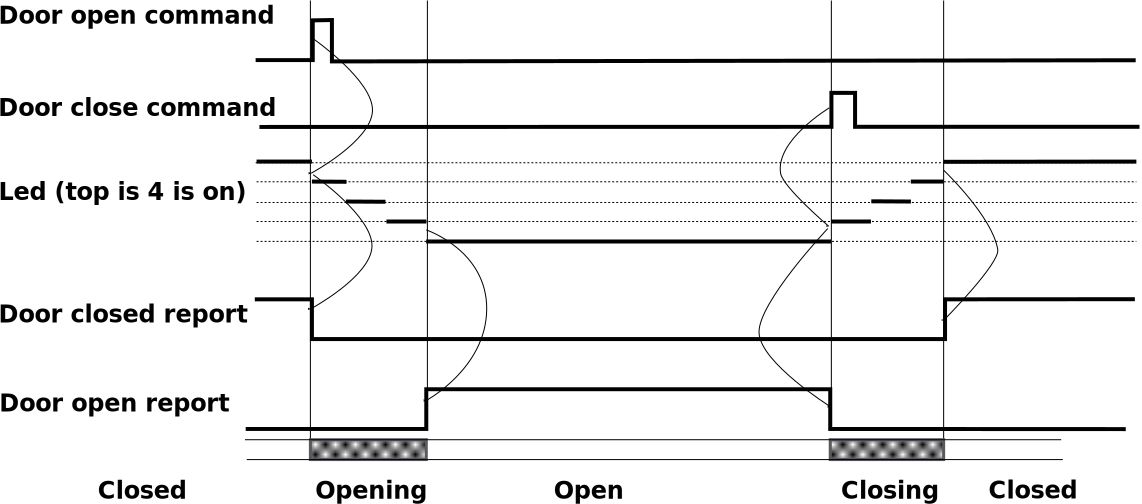
\includegraphics[width=\textwidth]{figures/doorsim}
  \caption{\label{fig:doortiming}Door timing diagram}
\end{figure}

\section{Input and outputs controlling the hardware model}

The elevator model is connected using the io-Warrior chip. This allows
control of 32 io bits. In the hardware 11 bits outputs and 21 bits are
used. The connections are listed in table~\ref{tab:connections} \vpageref[below]{tab:connections}.

\begin{table}[htbp]
  % \small
  \centering
  \caption{\label{tab:connections}Hardware connections of the elevator
    model}
  \shadowbox{
    \begin{tabular}{crcl}
      \textbf{in/out} & \textbf{bitNr} &\textbf{warrior bit}& \textbf{control} \\\hline
      in  & 0 & P0.0 & up button 0         \\
      in  & 1 & P0.1 & up button 1         \\
      in  & 2 & P0.2 & up button 2         \\
      in  & 3 & P0.3 & down button 1       \\\hline

      in  & 4 & P0.4 & down button 2       \\
      in  & 5 & P0.5 & down button 3       \\
      in  & 6 & P0.6 & door closed sensor  \\
      in  & 7 & P0.7 & red cage button (alarm button) \\\hline
      
      in  & 8 & P1.0 & target button 0     \\
      in  & 9 & P1.1 & target button 1     \\
      in  & 10 & P1.2 & target button 2     \\
      in  & 11 & P1.3 & target button 3     \\\hline

      in  & 12 & P1.4 & floor sensor 0      \\
      in  & 13 & P1.5 & floor sensor 1      \\
      in  & 14 & P1.6 & floor sensor 2      \\
      in  & 15 & P1.7 & floor sensor 3      \\\hline

      out& 16 & P2.0 & floor indicator light 0 \\
      out& 17 & P2.1 & floor indicator light 1 \\
      out& 18 & P2.2 & floor indicator light 2 \\
      out& 19 & P2.3 & floor indicator light 3 \\\hline

      out & 20 & P2.4 & Motor down bit       \\
      out & 21 & P2.5 & Motor up bit     \\
      out & 22 & P2.6 & door open cmd     \\
      out & 23 & P2.7 & buzzer (avoid)/blue led test   \\\hline\hline
\multicolumn{4}{c}{\textbf{Bits below are extensions on previous hardware}}\\\hline
      in  & 24 & P3.0 & (nurse button) (test)\\
      out & 25 & P3.1 & up led    \\
      out & 26 & P3.2 & down led   \\
      out & 27 & P3.3 & door close cmd \\\hline

      in  & 28 & P3.4 & door open sensor  \\
      in  & 29 & P3.5 & door open button \\
      in  & 30 & P3.6 & door close button \\
      in  & 31 & P3.7 & obstruction sensor \\\hline

\multicolumn{4}{p{80mm}}{\textbf{All bits are in true logic. A one
    activates LED or motor-bit, a 0 turns it off. For inputs: a 1 is
    an activated 
    sensor or button, a 0 is the inactive state.}}\\\hline
    \end{tabular}
  }
\end{table}

\begin{wrapfigure}{r}{60mm}
  \vspace{-1\baselineskip}
  \begin{center}
    \includegraphics[width=58mm]{figures/lift2.png}
  \end{center}
  \vspace{-1\baselineskip}
  \caption{Elevator model}
  \label{fig:lift}
  \vspace{-1\baselineskip}
\end{wrapfigure}
Notes: The door LEDs are not in the output list. They are controlled
with the door open and close command bits and can be monitored with the door
opened and closed sensor as can be seen in figure~\ref{fig:doortiming}
\vpageref[above]{fig:doortiming}. 

The elevator motor is controlled with two bits. It has two LEDs
connected, one for up and one for down, which light up when the motor
is switched on in that direction. The LEDs are on the bezel or
pedestal, out of sight of the passenger.

Left and right of the floor indicator lights on
each floor, there is one up and down LED. These LEDs should show the
travel direction chosen by the elevator control. These up/down LEDs
should go off when the elevator has no more calling or moving passengers.

In this project the hardware model is connected using the IO warrior
chip. This is then connected to the USB port of a computer (PC or
MAC). 

The inputs and outputs are pure binary, which allows  the use of one
bit for each of the inputs and outputs. An active bit has value 1 in
the aggregate, an inactive bit value 0.

\section{IO operations provided  by the IO Warrior}

The operations provided by the IO Warrior development kit can be found
in the Java documentation. For your convenience we provide a copy of
the IOwarrior software development kit  api at
\url{http://prj32.fontysvenlo.org/iowarrior-SDK/Java/doc/api/index.html}. 
The SDK can also be found at the prj32 web page \url{http://prj32.fontysvenlo.org/}.

To get you started and to remove some startup and shutdown issues we
provide a few utility classes in the package \lstinline{sevenlohwio}.
This package and some more packages is also available in the
project repository.


\subsection{Bit operations}
\lstset{language=Java}
The basic read and write operations on most computer binary IO is word
wide, in which the word with is 8, 16 or 32 bits at a time.
In most smaller systems, including the PC, the minimum amount is 8
bits or a byte. In the case of the IOWarrior we have an USB Human
intarface device. We use the IOWarrior in its simplest mode, in which
case its provides access to it IO pins with read and write of all the
32 bits at a time.
As an abstraction we define two interfaces that should implemented and
on which you can design and implement a complete binary IO subsystem.

The basic operations defined in the interfaces are 
\lstinline{int read()} and \lstinline{void write(int v)}. Implementing these
interfaces enables encapsulation of the IO device in classes. The
object of such an implementation class could for instance encapsulate
an IOWarrior or a network connection to an iowarrior connected to
another computer. The identification of the proper port and connector or
IOWarrior address should be taken care of in the constructor in the
class design, which assigns the port and card info to final fields.

Specific to the IOWarrior is that it behaves as a so called Human
Interface USB device, that is, it behaves similar to a keyboard or
mouse. This implies that a read operation only returns if there is
input. Such a operation is called a \textit{blocking} operation. 

Your main task in the project related to IO is to provide bit handling.
In particular you will have to implement the detection of the
input bit changes and notification of observers or listeners.
Of course you will have to design and implement the bit output
operations as well. 

We strongly suggest that you make use of a change-Listener design,
which is similar to an instance of the \Okis{Observer Pattern}
combined with \Okis{Adapter}. The listeners are then driven by a
method, \lstinline{void pollOnce()} defined in the interface 
\textbf{Poller} that periodically or regularly interrogates the 
input word.

In the class diagram in figure~\ref{fig:listener} you find part of the
hwio library. The white classes and interfaces are the ones that you
might want to extend or implement. In particular you will want to
implement \Code{BitListener}(s) and the \Code{AbstractBitFactory},
which produces \Code{InBit} and \Code{OutBit} Objects or derivatives
of thereof.
\begin{figure}[htbp]
  \centering
  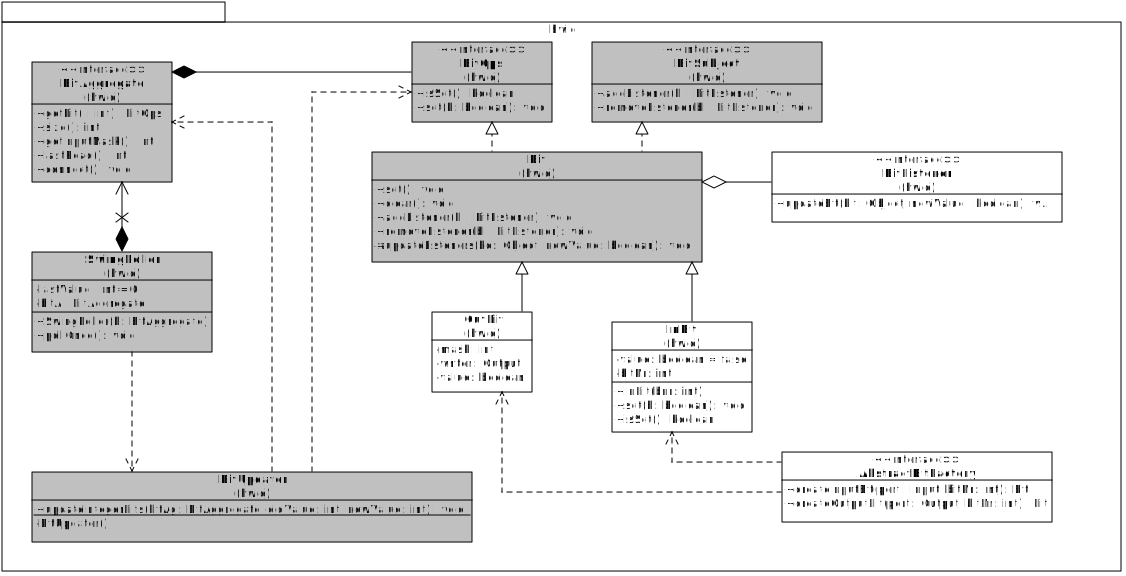
\includegraphics[width=\textwidth]{figures/hwio.pdf}
  \caption{Bit Listener class diagram of sevenlohwio}
  \label{fig:listener}
\end{figure}

\subsection{Bit handling}

To be able to isolate or operate on bits in word\footnote{Word is any
  group of bits in this context, in the examples you will see groups
  of 8, named octet or \lstinline{byte}, but \lstinline{short}, \lstinline{integer} and \lstinline{long} are also words
  in this context.} you need a few bitwise logical operation.

\begin{description}
\item[NOT] inverts all bits in a word, that is a 0
  becomes a 1 and a 1 becomes zero. Mathematical example:
  \texttt{
    \begin{eqnarray*}
      \begin{aligned}
        a      &=& 0101 & 0101\\\hline
        \lnot a &=& 1010 & 1010\\
      \end{aligned}
    \end{eqnarray*}}
  The Java (and C) symbol for the bitwise not operator is $\tilde{ }$ as
  in \lstinline{~a}.
\item[AND] a bit in the result is 1 if all the corresponding bits in
  all arguments are 1, else 0. Mathematical example:
  \texttt{
    \begin{eqnarray*}
      \begin{aligned}
        a         &=& 0100& 0101\\
        b         &=& 0001& 1111\\\hline
        a \land b &=& 0000& 0101\\
      \end{aligned}
    \end{eqnarray*}}
  The Java symbol is the single ampersand (\&) as in \lstinline{r = a & b}.
\item[OR] a bit in the result is 1 if the any of the corresponding bits in the
  arguments is one, else 0. Mathematical example
  \texttt{
    \begin{eqnarray*}
      \begin{aligned}
        a        &=& 0100& 0101\\
        b        &=& 0001& 1111\\\hline
        a \lor b &=& 0101& 1111\\
      \end{aligned}
    \end{eqnarray*}}
  The Java symbol is the single vertical bar ($|$)  as in \lstinline{r = a | b}.
  
\item[XOR] exclusive or. A bit in the result is 1 if exactly one of
  the corresponding bits is 1.
  \texttt{
    \begin{eqnarray*}
      \begin{aligned}
        a          &=& 0100& 0101\\
        b          &=& 0001& 1111\\\hline
        a \oplus b &=& 0101& 1010\\
      \end{aligned}
    \end{eqnarray*}}
  The Java symbol is the hat (\^\ )  as in \lstinline{r = a ^ b}. With two
  arguments the xor operation tells you which of the bits differ in the
  arguments.  
\end{description}

A summary of the logical operations with two one bit arguments is given
table~\ref{tab:logops}

\begin{table}[htbp]
  \caption{\label{tab:logops}Some logical operations}
  {    \renewcommand\arraystretch{1.7}
  \begin{tabular}{IccI>{\columncolor[gray]{.8}}cc>{\columncolor[gray]{.8}}cc>{\columncolor[gray]{.8}}cc>{\columncolor[gray]{.8}}cI}\whline
    \multicolumn{9}{IcI}{Logical operations (in bit wise programming notation)}\\\whline
    \multicolumn{2}{IcI}{semantics}
    & inverse & all (both) & at least one& unequal & equal & not all & none\\\whline
    \multicolumn{2}{IcI}{math sym}
      & $\neg a$ & $a\land b$         & $a\lor b$ & $a\oplus b$
      & $a=b$    & $\neg(a \land b)$ & $\neg(a \lor b)$ \\\whline
      \multicolumn{2}{IcI}{techn. not.}
      & $\overline{a}$ & $a\cdot b$ & $a+b$ & $a\oplus b$
      &$a=b$ & $\overline{a\cdot b}$ & $\overline{a+b}$\\\whline
      \multicolumn{2}{IcI}{C style. not.}
      & $\tilde{\ }a$ & $a \& b$ & $a|b$ & $a\hat{\ } b$
      &$a=\,=b$ & $\tilde{ }(a \& b)$ & $\tilde{ }(a|b)$\\\whline
    $a$ & $b$ & not(a) & and & or & xor & equals & nand & nor \\\whline 
    0 & 0 & 1      &  0  &  0 &  0  &  1     & 1    & 1   \\
    0 & 1 & 1      &  0  &  1 &  1  &  0     & 1    & 0   \\
    1 & 0 & 0      &  0  &  1 &  1  &  0     & 1    & 0   \\
    1 & 1 & 0      &  1  &  1 &  0  &  1     & 0    & 0   \\\whline
  \end{tabular}
}

\end{table}


\renewcommand\TheFile{gui.tex}
\SVN $Author: hom $
\SVN $Revision: 14 $
\SVN $Id: gui.tex 14 2013-05-13 13:36:54Z hom $
\SVN $Date: 2013-05-13 15:36:54 +0200 (Mon, 13 May 2013) $
\SVN $State: Exp $
\begin{savequote}[8cm]
  \sffamily
  All our dreams can come true, if we have the courage to pursue them.
  \qauthor{Walt Disney}
\end{savequote}
\chapter{Graphical user interface}

\parpic(60mm,45mm)[rs]{\includegraphics[width=58mm]{figures/gui-preview-02.jpg}}The current hardware model is somewhat limited and misses some
features that you would expect in a real elevator system.

To make the modelling more realistic we compensate for these missing
features in the graphical user interface.

You should use the Java Swing framework to implement the graphical
user interface of the system. There are a number of nice tutorials on
the web, such as \url{http://java.sun.com/docs/books/tutorial/uiswing}
at the Oracle/SUN website.

The document
\url{http://java.sun.com/products/jfc/tsc/articles/painting/} is 
very useful in understanding the architecture of painting in AWT and
swing.
 
\section{GUI features}

\paragraph{Lit buttons} In a modern elevator system you expect lit
buttons. Once a button is pressed, the button is lit. This light
stays on until the service requested by the passenger is
provided. As an example: when a passenger presses an UP button on
floor f, the button's light stays on until a cage visits floor f in
an upward journey. In the GUI presentation all buttons should have
lights.

\paragraph{Obstruction detection} A modern elevator, or any
automatically closing door for that matter, will have some kind of an 
obstruction sensor. In the GUI this sensor can be simulated by
implementing the GUI cage as some kind of button, in which the pressed
state equals obstruction.

\paragraph{Door Open and close buttons} A cage in an elevator system should
have an open and a close button, that requests the door to be opened
or closed. Once an elevator has a request which takes it to another
floor, the door is closed. If a cage stops at a floor a transfer
timeout must be observed, which can be shortened by pressing the door
close button and extended by pressing the door open button. Of course
the door should only open if the cage is at rest at a floor.

\parpic(60mm,35mm)[r]{\includegraphics[width=58mm]{figures/180dialbrassnumbers.jpg}}\paragraph{Cage position indication} As in the hardware model, the GUI
should also show the whereabouts of the cage on some kind of indicator
on each floor. The same approach as the hardware (two lights when
between floors) can be used. A dial model, such as used in old
fashioned elevator systems would be a very nice touch.

\paragraph{Multiple cages} A serious elevator system would have multiple
cages, making a strategy for up and down buttons more meaningful to
system and passengers. In your implementation you should be able to
support at least two cages in the GUI, where one of these GUI cages
will monitor the hardware elevator model. The idea is that this GUI cage
presents the behaviour of the hardware model, synchronous to that
model. You should try to make an attempt to let the GUI and the
hardware model move as synchronously as possible. The GUI cage will
have all the missing features as mentioned above and otherwise mimic
the hardware model faithfully. For instance if the red button is used
as the obstruct button, and the monitor provides obstruction
behaviour, then both the hardware cage and this monitor cage should
reopen its door and wait for the obstruction to be removed.  

\paragraph{Nurse button} The nurse button should also be present in
the GUI.

\paragraph{Number of floors} The GUI design should be able to support
at least 10 floors. 

\paragraph{Logging} The system should log all up and down requests and
arrivals as well as the motor cycles of all cages. (Up, down, stop).
The tail of this log (the last entries) should be shown in the GUI.

\paragraph{Floor announcement} Once the elevator stops at a floor due
to a target request, an audible floor announcement is given. In an
extended version of the system, this floor announcement may
have a different announcement signal for each floor. Simple but
distinct sounds can be used but thinkable is something like
\textit{``fourth floor, 
  penthouse and restaurant''}. The floor announcement system could
also be used to inform the passengers of special situations like out
of order messages and the like.



\renewcommand\TheFile{weekplan.tex}
\SVN $Author: hom $
\SVN $Revision: 23 $
\SVN $Id: weekplan.tex 23 2013-11-08 10:31:58Z hom $
\SVN $Date: 2013-11-08 11:31:58 +0100 (Fri, 08 Nov 2013) $
\SVN $State: Exp $
\begin{savequote}[8cm]
  \sffamily
  Genius is one percent inspiration and ninety-nine percent perspiration.
  \qauthor{Thomas A. Edison}
\end{savequote}
\chapter{Execution of the project}

\parpic(51mm,39mm){\includegraphics[width=51mm]{figures/WorkinProgress.jpg}}The
main focus of this project is on reactive systems and usage of
design patterns. This explains why we enforce a rather strict plan, to
make sure that all goals are met and groups do not get into trouble
due to inadequate planning. Note that the planing is quite tight. So
not only work as a team towards the next delivery (there is one every
week), but properly use all available manpower. That is: Near a
delivery deadline most of your team members should be done with the
work for that deadline and 2 project members are  involved in preparing
the demo for the deadline. The others should be working on
investigating the deliverables for the next deadline.

\section{Products}

The products of this assignment are:
\begin{enumerate}
\item Report
\item Model
\item Implementation
\end{enumerate}

\subsection{How to deliver your assignment products}
All electronic products must be handed in via \href{https://www.fontysvenlo.org/peerweb}{peerweb}. See peerweb for all deadlines.
\begin{enumerate}
\item Report: one document describing your analysis, design and its
  implementation, test installation and user manual to be handed in on
  paper too, \emph{properly bound at the copy shop}. The document should also
  contain a reference to the repository. 
  See the weekly plan for what the document should contain. The
  design diagrams, user interface illustrations etc. are copied into
  and explained in the report document. In the document code fragments
  are shown only when relevant. E.g.  when the implementation is
  discussed in the describing text.
\item  Models: One model file in the Visual Paradigm UML tool.
  The models should contain analysis, design and implementation as
  well as a reverse engineered model of the complete
  implementation. For practical reasons you may use more then one
  model file for each of the phases analysis, design and
  implementation. You may hand in three distinct models.
\item Implementation: All (re)sources needed to build the project
  should be in the project repository at all times. The sources should
  be accompanied with an ant build script. Most of the time the
  Netbeans build.xml script will do.
  
  For all but the first week you should produce a executable artefact
  or runnable program. 
  By checking out the project and calling ant jar should result in a
  functional and runnable jar file. Say the produced jar file is
  called \Okis{dist/SuperElevator.jar}
  I will use the file like this:\\
  \frame{\scriptsize\Code{java~-cp~dist/SuperElevator.jar~nl.fontys.sevenlo.prj32.DemoWeekX}}.
  
  The prefix \Code{nl.fontys.sevenlo.prj32} is mandatory for all your
  packages. You may (maybe should) have additional packages under this
  top package name. You may also create several Netbeans projects with
  additional package and directory structures to reflect your
  functional decomposition.
  
  Each week that has an executable will have a Main class named\\
  \Code{nl.fontys.sevenlo.prj32.DemoWeek\textit{\textbf{weeknr}}}. For each
  week, except the first, there will be a hand in of a runnable jar file.
\end{enumerate}

\section{Naming conventions}
\paragraph{Libraries}
You will be using supplied libraries for the control of the
hardware. You may look at it as a layered architecture. The hardware
layer is provided by the \Code{IOWarrior} Library. It is provided by
the manufacturer of the IOWarrior chip, Code Mercenaries GmbH.

The bit io abstraction layer is provided by \Okis{sevenlohwio}
library. It provides a bit wise io abstraction.

The \Okis{sevenlowarrior} combines the facilities provided by the
hardware with the abstraction layer and thus provides USB based
bitwise io. 

For testing purposes in a gui environment sevenlowarrior uses the
\Okis{sevenlowidgets} library. Aside the use for iowarrior testing it
also provides some goodies that can be use full in your elevator
implementation.

The widgets library itself uses some resources that must be loaded
from the class path. We use \Okis{sevenloutils} for that.

To be able to use these libraries in a platform and java/netbeans installation
independent way, create netbeans libraries.


You get most comfort if you install the libraries complete with source
and javadoc. 

The names of these libraries and the installation\footnote{The paths
  used are for Debian/Ubuntu Linux.} steps as netbeans library are:
{
\setlength\parsep{0pt}
\setlength\topsep{0pt}
\setlength\partopsep{0pt}
\setlength\parskip{0pt}
\setlength\itemsep{0pt}
\newcommand\Classpath{[Classpath]}
\newcommand\Sources{[Source]}
\newcommand\Javadoc{[Javadoc]}
\begin{description}
\item[CodeMercenaries] The hardware access layer.
  \begin{description}
  \item[\Classpath] The library proper is at \Code{/usr/share/java/codemercs.jar}.
  \item[\Sources] Add the file \Code{/usr/share/java/codemercs-src.jar}.
  \item[\Javadoc] Add the file \Code{/usr/share/java/codemercs-doc.zip}.
  \end{description}
\item[SEVenloHWIO] The bit io abstraction layer. 
  \begin{description}
  \item[\Classpath] The library proper is at \Code{/usr/share/java/sevenlohwio.jar}.
  \item[\Sources] Add the file \Code{/usr/share/java/sevenlohwio-src.jar}.
  \item[\Javadoc] Add the file \Code{/usr/share/java/sevenlohwio-doc.zip}.
  \end{description}
\item[SEVenloWarrior] The bit io abstraction layer. 
  \begin{description}
  \item[\Classpath] The library proper is at \Code{/usr/share/java/sevenlowarrior.jar}.
  \item[\Sources] Add the file \Code{/usr/share/java/sevenlowarrior-src.jar}.
  \item[\Javadoc] Add the file \Code{/usr/share/java/sevenlowarrior-doc.zip}.
  \end{description}
\item[SEVenloWidgets] The gui widgets. 
  \begin{description}
  \item[\Classpath] The library proper is at \Code{/usr/share/java/sevenlowidgets.jar}.
  \item[\Sources] Add the file \Code{/usr/share/java/sevenlowidgets-src.jar}.
  \item[\Javadoc] Add the file \Code{/usr/share/java/sevenlowidgets-doc.zip}.
  \end{description}
\item[SEVenloUtils] The resource utils. 
  \begin{description}
  \item[\Classpath] The library proper is at \Code{/usr/share/java/sevenloutils.jar}.
  \item[\Sources] Add the file \Code{/usr/share/java/sevenloutils-src.jar}.
  \item[\Javadoc] Add the file \Code{/usr/share/java/sevenloutils-doc.zip}.
  \end{description}
\end{description}
} % end of lengths
All these libraries can be found at the module website.

To ease your getting into the matter, we've created a project in GIT,
containing a sub directory containing a maven netbeans project, called
bitfactoryexample. You can clone it with the coordinates
\texttt{git@fontysvenlo.org:2013/prj32m1/g4}. You should be able to
  build and run this project. The command line way to build it is
\texttt{mvn compile assembly:single}, which will build a singe jar
containing all the required libraries. This maven command should pull
in all the required resources and libraries.

If you also would like to get the sevenlo libraries described
above. Clone the repository \texttt{git@fontysvenlo.org:2013/prj32m1/g4}.



\subsection{Group repository}
\parpic[rs]{\includegraphics[width=39mm]{figures/projecttree.png}}The
repository contains a predefined directory structure. All source 
code (including tests) should be placed under \Code{sources}. The \Code{doc}
directory is intended for the documentation including the analysis and
design models. Use Visual Paradigm for your UML modelling. It also
integrates quite well with subversion\footnote{with git I do not know} through its \textit{team work}
capabilities. The doc directory strongly hints at preparing your
report using \LaTeX.

\paragraph{Project name} The netbeans projects shall be named with a
group prefix in front of them in the form of \Okis{gx\_}, where \textit{x} is
one of 01\ldots04  as in \Code{g01\_elevator}.

This also applies if you split your whole project into several
(netbeans) sub-projects for instance for specific subsystems. This is
a good idea anyway. So you might have a \Code{g01\_guiwidgets} library
project.

At the end you will have to deliver the complete deployable binary in
a zip file. This zip file will have the name gx\_elevator.zip. This
zip file must contain all that is needed to deploy the applications
via web start, using the jnlp protocol. The zip file should contain all
that is packed into the \Code{dist} subdirectory, including the dist
subdir itself. In \Linux that would be the \\
\framebox{\Code{zip -r g01\_elevator.zip dist}}\\
-command.

Tagging and branching of the documentation (doc) subtree is not required.
However the sources subtree will be tagged each week (see below).

A tag (and a branch) are simple copy commands in subversion. See the
appropriate documentation in the svnbook at
\url{http://svnbook.red-bean.com/en/1.5/svn.branchmerge.tags.html}. Use
the appropriate source and destination urls and all is done on the
server with minimal delay. Being versed at the subversion command line
is very rewarding here. If not sure, try things first in your
personal scratch pad repository.

In git, tagging is simple too, See \url{http://git-scm.com/book/en/Git-Basics-Tagging}.

\paragraph{Tags} Each week the tutors will make a TAG with the name
pattern TAG\_WEEKx. Other TAGS may be used freely.

\paragraph{Branches} You develop on the trunk, which is where the most
project members are working. Near a deadline, some will be preparing
for the demo of that period. Consider using a branch for the last
preparations so that work by others does not inter fear with your demo
project. From there pick up the stuff from the trunk in a controlled
way by applying the proper \Okis{merge} commands from trunk.
Consider branch names like \Okis{LOGIC\_RELEASE} etc.

In Git you do not need branches for a local experiment, as long as you
do not push the incomplete experiment results to the origin.

\paragraph{Final delivery} The final deliveries are: reports in pdf file format and a java
web start enabled jar bundle. Making a web start-able project in netbeans is fairly easy. 
Use the project properties and enable web start, Select
\begin{Itemize}
\item \textbf{[Codebase]:}  \texttt{User defined (e.g. HTTP Deployment)}, and
\item \textbf{[Codebase Preview:]}  \texttt{\scriptsize
    http://prj32.fontysvenlo.org/2011/gx\_elevator/dist/launch.jnlp},
  substituting x with your group number. Running \texttt{ant jws-run}
  with these settings will fail locally, but will produce a correctly populated
  \Code{dist} subdirectory.
\end{Itemize}


\section{Weekly planning}
The weekly rhythm must be strictly observed. The hand in for all but
the last deliverable will all be done using subversion to the URL
for your group as mentioned on the PRJ32 website. As hand in time the
svn time is taken. Note that this always is UTC, thus not the same as
your wall clock time.

During all project weeks you will keep a time record of all
the time spent on the project.

At the end of each project week the tutor will tag the repository with
a read only tag for all groups. The material in the tag is considered
handed in. The rest is not.

\setlength\extrarowheight{4pt}
\begin{longtable}{|p{10mm}|p{20mm}|p{90mm}|}%
  \caption{Week plan}\\\hline%
  \rowcolor[gray]{0.8}\textbf{week}&\textbf{delivery}&\textbf{Task and
    product}\\\hline%
 \endhead%
  \hline \multicolumn{3}{r}{\emph{week plan continued on next page}} 
 \endfoot%
  \hline \multicolumn{3}{c}{\textbf{End of week plan}}%
 \endlastfoot%

  1 & \begin{minipage}{18mm}
    SCM \\ TAG~WEEK1 
  \end{minipage}
  &  \begin{minipage}{90mm}
    \RaggedRight
    \vspace*{3mm}
    {\large\textbf{Analysis}}
    \begin{description}
    \item[Use case description] describing the main success
    scenarios (including the alarm scenario). (Hint: subdivide the
    journey into 4 sub scenarios; there is also an alarm scenario). 
  \item[Use case diagrams] showing the relations between the use cases.
  \item[Analysis class diagram] including CRC descriptions of the
    classes
  \item[Sequence diagrams] of the main scenarios. If you followed the
    advice in the use cases you should have 5 sequence diagrams.
  \item[State model] The system obviously has state behaviour. Model
    this state behaviour of the system and its subsystems using  state
    diagrams.
  \item[Data model] Data model is a posh\footnote{Posh is the not so posh word for chique} word for how to keep track of
    all requests and commands of the elevator system. Design a data
    model with appropriate operations. The data model may keep up and
    down requests separate from target requests. From the start think
    of multiple shaft systems.
    \end{description}
    
  \end{minipage}\\\hline
  2 & 
  \begin{minipage}{18mm}
    SCM\\ TAG~WEEK2
  \end{minipage}
  & \begin{minipage}{90mm}
    \RaggedRight
    \vspace*{3mm}
    {\large\textbf{Hardware subsystem and Data model}}
    Analysis, design and implementation of the hardware IO
    subsystem. The hardware elevator will be connected using USB and a
    small IOWarrior printed circuit board. You will be given the complete
    IOWarrior library (which is available from code mercenaries) plus a
    library that provides the elementary read and write operations to the
    hardware.
    
    Deliverables:
    \begin{description}
    \item[Class model IO subsystem] A complete design class model of the
      system. For the report you will need diagrams of the subsystems.
    \item[Implementation of IO subsystem] As usual: no implementation is
      complete without tests.
    \item[Data model and implementation] including tests of all the
    operations.
    The test on the data model \textbf{must} have 100\% statement
    coverage, to be determined with the Emma coverage plug in.
    \end{description}
  \end{minipage}
  \\\hline
  3 & \begin{minipage}{18mm}
    SCM\\  TAG~WEEK3
  \end{minipage}
  & \begin{minipage}{90mm}
    \RaggedRight
    \vspace*{3mm}
    {\large\textbf{GUI and simulation}} design and design and
    implementation of the widgets used in this design.
    
    Deliverables:
    \begin{description}
    \item[Drawing of the gui design] I would use inkscape. You might
      want to opt for Adobe Illustrator or a similar tool. Make sure
      you are able to deliver a vector type file. (SVG or PDF).
    \item[Widgets] The \textbf{Cage} which should provide obstruction detection
      functionality. \textbf{Up} and \textbf{down} buttons including
      the appropriate. \textbf{Floor sensor indicators} which show
      when a floor sensor is activated. 
      \textit{ButtonModels}. Target buttons. Note that all these
      widgets get rather little real estate in the GUI picture.
    \item[State machine](s) implementation  for the behaviour of the system. 
    \end{description}
    
  \end{minipage}
  \\\hline
  4 & \begin{minipage}{18mm}
    SCM\\TAG~WEEK4
  \end{minipage}
  & \begin{minipage}{90mm}
    \RaggedRight
    \vspace*{3mm}
  {\large\textbf{Data model and  GUI  integration}}
  
  Deliverables:
  \begin{description}
  \item[Integrated GUI simulation] that shows the functionality
    of the widgets and the whole system so far. This simulation
    should already behave like a normal elevator system with
    respect to state behaviour. The data model should be used.
  \item[Strategy design] Use the Strategy pattern to implement
    different behaviours of the system in several modes. Implement
    one simple but useful strategy.
    
    \end{description}    
  \end{minipage}
  \\\hline
  5 & \begin{minipage}{18mm}SCM \\TAG~WEEK5
  \end{minipage}
  & \begin{minipage}{90mm}
    \RaggedRight
    \vspace*{3mm}
    {\large\textbf{GUI - hardware integration}} with simple strategy.
    \begin{description}
    \item[Combined hardware and software model] in which the GUI shows
      two cages, one simulation and the other as a monitor to the
      hardware model. This implementation must be working for a
      building with 4 floors.
    \end{description}
    \vspace{.3\baselineskip}
  \end{minipage}
\\\hline
  6 & SCM TAG~WEEK6 & \begin{minipage}{90mm}
    \RaggedRight
    \vspace*{3mm}
    {\large\textbf{Additional strategy implementations}}
    \begin{description}
    \item[Strategy] implementations for the remaining operating modes.
    \end{description}
    {\large\textbf{Documenting, presentation and demo preparation}}
    \begin{description}
    \item[Complete class documentation] extract-able with javadoc.
    \item[all diagrams] for the report.
    \item[Report] with sections \textbf{requirements},
      \textbf{analysis}, \textbf{design}, \textbf{implementation
        details}, \textbf{test plan} describing what you intended to
      test, \textbf{deployment manual} and a \textbf{User manual}.
    \end{description}
    \vspace{.3\baselineskip}
  \end{minipage}
\\\hline
  7 & \begin{minipage}[b]{18mm}
    SCM + peerweb\\TAG~WEEK7\\
    +reports (.pdf) \\
    in peerweb
    \\
    presentation \\and\\ demo
  \end{minipage}
  & \begin{minipage}{90mm}
    \RaggedRight
    \vspace*{3mm}
    {\large\textbf{Delivery week}} in which the products are
    presented and demonstrated. During this demonstration the use of
    compilers, editors and the like is forbidden. All code should be
    runnable in delivered binary form. For Java that would be a jar
    file, possibly combined with a startup script. You may use several
    startup scripts to show different features of your application,
    but all  should use the same (set of) jar file(s).

    All groups will provide a zip file that contains an application
    that is deployable through a web site using Java web start. This
    zip file must be self contained and have no external dependencies
    that have to be pre-installed. This should provide  us to have
    very nice set of demo applications. See the netbeans documentation
    on how to do that. This application should be able to work with
    and without the iowarrior drivers and libraries installed. 

    All students must attend the presentation demonstration of all
    groups.

    \begin{description}
    \item[Final execution report] Time usage sheets for all group
      members summarised over the whole project. 
    \item[Defects report] Defects found during tests and integration
      with an impact analysis. An impact analysis describes what the
      subsequent effect of this defect is on the rest of or the
      overall system .
    \end{description}
  \end{minipage}
  \\\hline
\end{longtable}  

\addcontentsline{toc}{section}{Bibliography}
\bibliography{sebivenlo}
\section*{Colofon}

The original hardware model is provided by Hogeschool Rotterdam.

The model currently is use has undergone several revision. The latest model has been built with a USB only connection, with added hardware functionality (full door control, open/close buttons, test obstruction and nurse button) is a idea of Pieter van den Hombergh.

The electronics and the new mechanics has been designed and built  by VeTeTronics B.V., Tegelen. The drawing of the model on page \pageref{fig:lift} is made by Denny Beulen.

The design and manufacturing of the box at the underside has been
produced by Jochem Högerle at the Fontys Hogeschool voor Techniek and
Logistiek laboratory for mechanical production. 

The software libraries are designed and maintained by Pieter van den Hombergh.


\fancyhf{} % clear all
\renewcommand\headrule{}
\renewcommand\footrule{}
\nolinenumbers
%\setlength\oddsidemargin{0pt}
\newpage
\cleartoevenpage
\setlength{\unitlength}{1mm}
\fancyhead[LE]{
  \begin{picture}(0,0)(20,275)
    \put(5,0){\fbox{
\includegraphics[width=216mm]{figures/fontys-page}}}
    \put(100,285){\color{fontys}\sf\Large{Fontys Venlo Software
        Engineering series}}
    \put(15,0){\includegraphics{figures/barcode}}
  \end{picture}
}

\newpage

\vspace*{40mm}
\begin{center}
  \begin{picture}(160,180)(-10,0)
    \put(-40,140){\includegraphics[width=65mm]{figures/elevator1.jpg}}
    \put(40,20){\includegraphics[width=105mm]{figures/lift2.png}}
  \end{picture}
\end{center}

\end{document}
